\documentclass[10pt]{article}
\usepackage[margin=0.70in]{geometry}
\usepackage{amsmath,amssymb}
\usepackage{booktabs,graphicx,tabularx,enumitem}
\usepackage[T1]{fontenc}
\setlength{\parindent}{0pt}
\setlength{\parskip}{4pt}
\setlist[itemize]{leftmargin=1.25em,noitemsep,topsep=2pt}
\newcommand{\du}{\Delta u}
\begin{document}

\begin{center}
{\Large\bfseries Hybrid PAX--Photodiode Locking for $\phi_1$: Checkpoint Method and Results}\\[2pt]
{\small Experimental checkpoint, 15 August 2026}
\end{center}

\textbf{Purpose.} This checkpoint records the most repeatable current method for holding the $\phi_1$-controlled Poincar\'e-sphere azimuth. It is a \emph{framework report}: the PAX monitor and photodiode (PD) may move in the full apparatus, so the measured local gains must be recalibrated, but the two-loop architecture and safety logic transfer directly.

\section*{1. Control architecture}
The PAX supplies Stokes estimates $(S_1,S_2,S_3)$ and the experimental azimuth is
\begin{equation}
 u=\operatorname{atan2}(S_3,S_2), \qquad e_u=\operatorname{wrap}(u_\star-u).
\end{equation}
The PAX is deliberately not the fast actuator sensor. A PD at the final-output port supplies the fast error signal, while the PAX corrects the slow bias that makes a fixed PD level correspond to a changing polarization state. Figure~\ref{fig:architecture} shows the separation of roles.

\begin{figure}[h]
\centering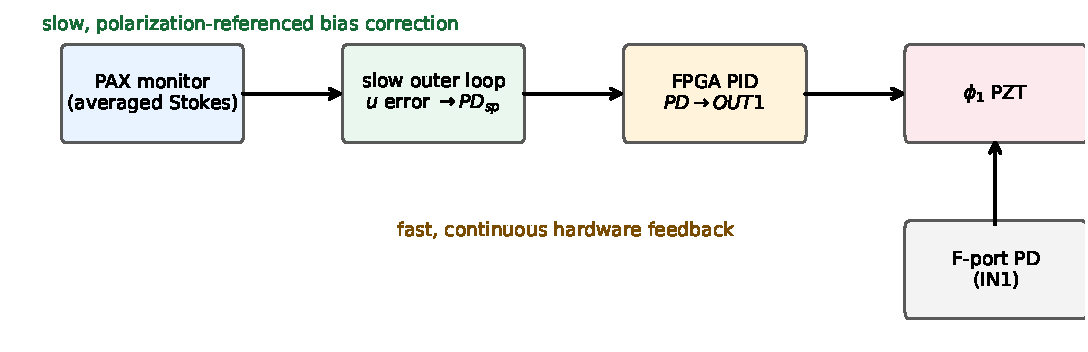
\includegraphics[width=.98\linewidth]{figures/architecture.pdf}
\caption{Hybrid control allocation. The FPGA PID drives $OUT1\rightarrow\phi_1$ continuously; PAX changes only the FPGA PD setpoint at low bandwidth.}
\label{fig:architecture}
\end{figure}

At each fresh local operating point, held sweeps measure
\begin{equation}
 a=\frac{dPD}{dV_{OUT1}},\qquad b=\frac{du}{dV_{OUT1}}.
\end{equation}
The signed FPGA proportional term is chosen for negative feedback, $P=-\operatorname{sgn}(a)|P|$, and its magnitude is set by a normalized local loop gain $|Pa|=0.22$. The integral unity-gain frequency is $5$~Hz. The integrator is seeded at the present output, and a 1~s P-only check rejects a rail before integral action is enabled.

Every $T_o=3$~s, an average of three PAX Stokes records updates the PD setpoint:
\begin{equation}
 PD_{sp,k+1}=PD_{sp,k}+\operatorname{clip}\!\left[
 g_o e_{u,k}\frac{a}{b},\; -1.5\ \mathrm{mV},\;+1.5\ \mathrm{mV}\right],
 \quad g_o=0.12.
\end{equation}
Since $du/dPD=b/a$, this converts a measured polarization error into the PD-setpoint shift that the FPGA must realize. Crucially, this is a \emph{setpoint} trim: PAX never writes sparse voltage steps to the piezo.

\section*{2. Repeated short-hold evidence}
Three independent 27~s holds using the settings above were selected because each completed under the autonomous experimental runtime limit and used fresh local calibration. The combined 30 PAX validation samples give a median $|\du|=0.0329$~rad, 90th percentile $0.131$~rad, and median PD residual $1.59$~mV. The distribution is centered ($\overline{\du}=-0.0077$~rad), which is the key improvement over PD-only holds that could retain a substantial polarization bias.

\begin{figure}[h]
\centering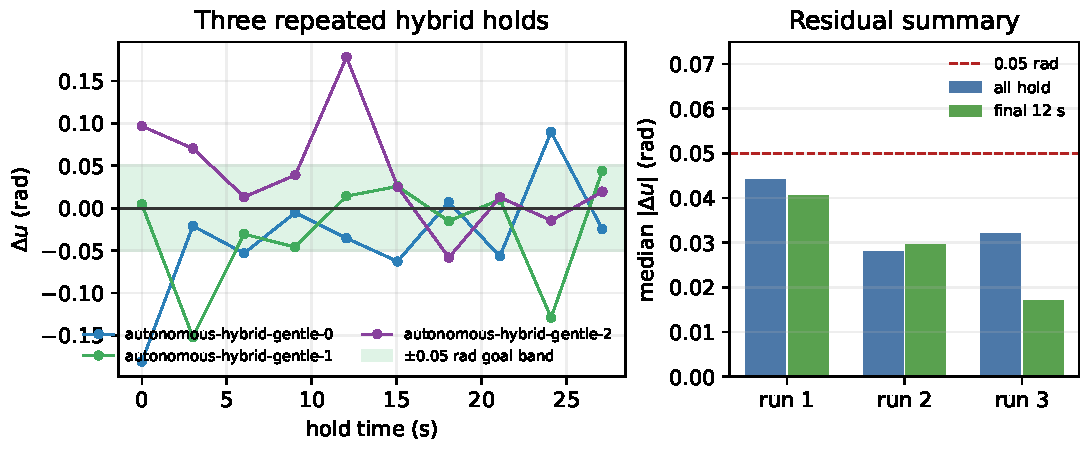
\includegraphics[width=.98\linewidth]{figures/results.pdf}
\caption{PAX validation of the retained hybrid method. The $\pm0.05$~rad band is a useful current target, not a claim of guaranteed long-duration performance.}
\label{fig:results}
\end{figure}

\begin{center}
\begin{tabular}{lccc}
\toprule
Trial & median $|\du|$ & final-window median & fraction $|\du|<0.05$ rad\\
\midrule
gentle-0 & 0.044 rad & 0.057 rad & 0.50\\
gentle-1 & 0.028 rad & 0.026 rad & 0.80\\
gentle-2 & 0.032 rad & 0.020 rad & 0.60\\
\bottomrule
\end{tabular}
\end{center}

\section*{3. Transfer and retuning protocol}
When either detector location changes, do not reuse the voltage-to-polarization or PD calibration numbers. Reuse the following sequence instead:
\begin{enumerate}[leftmargin=1.5em,noitemsep]
\item Place the system at the intended branch and run a fresh held $\phi_1$ sweep. Confirm a locally monotonic PD flank and an appreciable $b=du/dV_{OUT1}$.
\item Measure $a$ and $b$ at that same branch. Set the sign of $P$ from $a$; begin with a conservative normalized gain below $|Pa|=0.22$ and $I=0$ during handoff.
\item Seed the FPGA integrator with the present output, perform the P-only rail check, then enable a low integral gain. Confirm that PAX u remains on the selected branch.
\item Enable the PAX outer trim with low gain and bounded PD-setpoint steps. Tune outer bandwidth only after the inner PD loop is stable; score changes by PAX $|\du|$, not PD error alone.
\end{enumerate}

\textbf{Checkpoint conclusion.} The experiment supports a practical division of labor: the PD/FPGA loop suppresses fast optical drift with smooth actuator output, while the slow PAX loop removes the otherwise persistent PD-to-polarization bias. The reported sub-$0.05$~rad short-hold results are promising and repeatable, but a separate 120--180~s confirmation remains required before claiming long-duration stability.

\end{document}
